\subsection{定位和图像分割}
这一章节的总流程图,见图\ref{fig-steps}。
\begin{figure}[htbp]
    \centering
    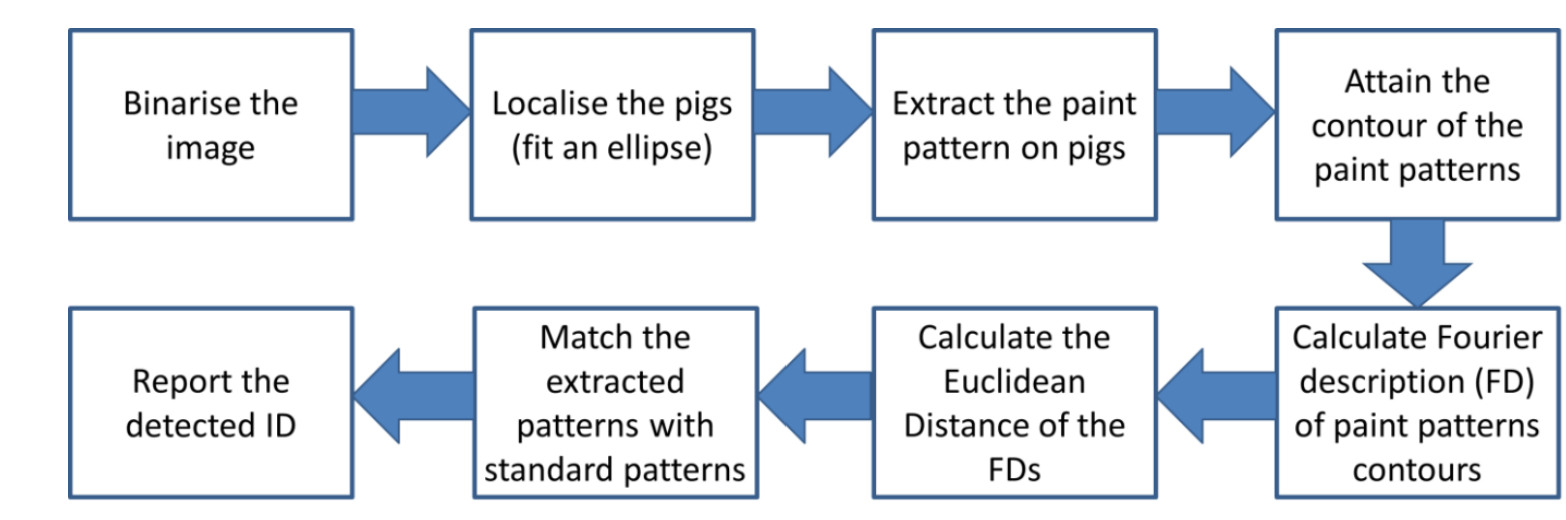
\includegraphics[width=0.9\textwidth]{pic/steps.png}
    \caption{流程概述,初步图片,待修改}
    \label{fig-steps}
\end{figure}

\subsubsection{初步裁剪}
首先,对图片进行初步分割,确定喂食器和猪圈地板的位置。确定地板的范围后,我们将图片边缘处相机机盖裁剪去除。由于喂食器的色泽与猪的身体相近,将其排除也有助于提高后续检测的准确率。
\begin{figure}[htbp]
    \centering
    \begin{minipage}{0.49\linewidth}
        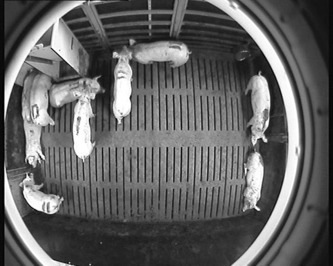
\includegraphics[width=0.9\linewidth]{pic/before_cut.jpg}
        \caption{裁剪边框前}
        \label{fig-before_cut}
    \end{minipage}
    \begin{minipage}{0.49\linewidth}
        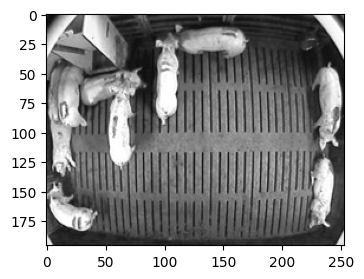
\includegraphics[width=0.9\linewidth]{pic/after_cut.png}
        \caption{裁剪边框后}
    \end{minipage}
    \label{fig-cut}
\end{figure}


\subsubsection{基于局部自适应直方图均衡的对比度加强}
为了加强提取轮廓的效果,需要先增加图片的对比度。这里我选择了局部自适应的直方图均衡算法(regionally adaptive histogram equalization)。

先介绍传统的全局直方图均衡算法的数学原理,以单通道的灰度图片为例。假设图片灰度值可取$\{0, 1, \dots, L-1\}$,大小为$M\times N$,记灰度值为$i$的像素点数量为$n_i$,则有$MN=\sum_{i=0}^{L-1}n_i$。归一化直方图的对应分量$p_i=\frac{n_i}{MN}$。设输入像素点的灰度为$i$,则输出的灰度为$T(i)$
\begin{equation}
    T(i) = \lfloor (L-1) \sum_{j=0}^i p_j \rfloor
    \label{discrete global HE}
\end{equation}

假如$L$足够大时,我们可将离散的灰度$i$近似处理为连续变量。从图片中随机取一点,记对应的连续随机变量为$X\in[0,L]$,概率密度函数为$p(x)$。式(\ref{discrete global HE})对应的

然而传统的全局直方图均衡算法有明显的缺点。xxx

而局部自适应的xxx,其方法如下。

\subsubsection{基于Otsu算法的图像二值化}
用Otsu算法选择阈值,将灰度图片转化为二值图片。Otsu法能最大化二值分类的类间方差,且只用到图片的灰度直方图。其原理如下。

设$M,N,n_i,p_i,L$的定义与之前章节一致。从图片中随机选取一个像素点,记其灰度值为随机变量$I$,则$\Pr(I=i)=p_i$。

若选择阈值$T(k)=k\in N$,使得灰度属于$[0,k]$的像素点被分类为$c_1$,灰度属于$[k+1,L-1]$的像素点被分类为$c_2$。则像素点属于$c_i$的概率为
\begin{eqnarray}
    \Pr(c_1,k) &=& \sum_{i=0}^k p_i \\ 
    \Pr(c_2,k) &=& 1 - \Pr(c_1,k)
\end{eqnarray}
这样的分类与$k$有关,但为了符号上的简洁,以下将参数$k$略去,例如$\Pr(c_i):=\Pr(c_i,k)$。

属于$c_1$时,由贝叶斯公式,$I$的条件期望为
\begin{equation}
    \E(I|c_1) = \sum_{i=0}^k i \Pr(i | c_1) 
    = \frac{1}{\Pr(c_1)} \sum_{i=0}^k i p_i
\end{equation}
类似地,属于$c_2$时的条件期望为
\begin{equation}
    \E(I|c_2) = \frac{1}{\Pr(c_2)} \sum_{i=k+1}^{L-1}i p_i
\end{equation}
显然,条件期望和期望满足
\begin{equation}
    \E(I) = \sum_{i=1,2} \Pr(c_i) \E(I|c_i)
\end{equation}

我们定义类间方差为
\begin{equation}
    \sigma_B^2 = \sum_{i=1,2} \Pr(c_i) [ \E(I|c_i) - \E(I) ]^2
\end{equation}
,而Otsu算法选择的阈值$k_{Otsu}$即最大化类间方差
\begin{equation}
    k_{Otsu} = \arg \max_{k\in N, 0\leq k <L} \sigma_B^2 (k)
\end{equation}
再根据计算得到的阈值将输入灰度图片$f(x,y)$变换为黑白图片$g(x,y)$
\begin{equation}
    g(x,y) = \begin{cases}
        1, & f(x,y) > k_{Otsu} \\
        0, & \text{otherwise}
    \end{cases}
\end{equation}

\subsubsection{基于椭圆拟合的图像分割}


\subsection{ID检测}
\subsubsection{提取ID标识}
\subsubsection{基于傅里叶变换的ID匹配}

\subsection{体重估计}
\subsubsection{线性回归分析}
